% !TeX program = pdflatex
\documentclass[10pt,aspectratio=169]{beamer}

% ---------------------------------------
% Langue & encodage
% ---------------------------------------
\usepackage[utf8]{inputenc}
\usepackage[T1]{fontenc}
\usepackage[french]{babel}
\usepackage{lmodern}

% ---------------------------------------
% Maths & utiles
% ---------------------------------------
\usepackage{amsmath, amssymb, mathtools}
\usepackage{physics}
\usepackage{siunitx}
\usepackage{graphicx}
\usepackage{booktabs}
\usepackage{tikz}
\usepackage{hyperref}

% ---------------------------------------
% Couleurs & thème minimal
% ---------------------------------------
\definecolor{Primary}{HTML}{6C5CE7}   % mauve-bleuté
\definecolor{Secondary}{HTML}{A39BFF} % plus clair
\definecolor{Accent}{HTML}{2D9CDB}    % bleu accent discret
\definecolor{Dark}{HTML}{1F2430}
\definecolor{Light}{HTML}{F6F7FB}

\setbeamercolor{normal text}{fg=Dark,bg=white}
\setbeamercolor{structure}{fg=Primary}
\setbeamercolor{title}{fg=white,bg=Primary}
\setbeamercolor{frametitle}{fg=Primary,bg=Light}
\setbeamercolor{block title}{fg=white,bg=Primary}
\setbeamercolor{block body}{bg=Light}
\setbeamercolor{itemize item}{fg=Primary}
\setbeamercolor{itemize subitem}{fg=Secondary}
\setbeamercolor{page number in head/foot}{fg=Primary}

\setbeamertemplate{navigation symbols}{} % pas d'icônes
\setbeamertemplate{frametitle}{
  \vspace{2pt}
  \begin{beamercolorbox}[wd=\paperwidth,sep=5pt,leftskip=10pt]{frametitle}
    \usebeamerfont{frametitle}\insertframetitle
    \ifx\insertframesubtitle\@empty\relax\else\\[-2pt]
      \usebeamerfont{framesubtitle}\footnotesize\insertframesubtitle
    \fi
  \end{beamercolorbox}
}

% Pied de page minimal avec numérotation
\setbeamertemplate{footline}{
  \leavevmode
  \hbox{\hspace*{\dimexpr\paperwidth-1.8cm\relax}
    \begin{beamercolorbox}[wd=1.6cm,ht=2.8ex,dp=1ex,center]{page number in head/foot}
      \insertframenumber/\inserttotalframenumber
    \end{beamercolorbox}}
  \vspace{0.2ex}
}

% Plan en début de section
\AtBeginSection[]{
  \begin{frame}{Plan}
    \tableofcontents[currentsection]
  \end{frame}
}

% ---------------------------------------
% Métadonnées
% ---------------------------------------
\title[ PFE — ENSTA Paris ]{Stratégies modernes pour l'intégration des équations d'advection–réaction–diffusion\\
{\small (ImEx \& Multi\-Résolution Adaptative)}}
\author[Alexandre EDELINE]{\textbf{Alexandre EDELINE}}
\institute[ENSTA Paris \& CMAP]{
  ENSTA Paris \\
  Laboratoire: CMAP \\
  Tuteurs laboratoire: Marc MASSOT, Christian TENAUD \\
  Tuteur ENSTA: Patrick CIARLET
}
\date{Avril — Septembre 2025}

% Optionnel : logos (placez vos fichiers dans figs/)
\titlegraphic{%
  \vspace{-2cm}
  
\includegraphics[height=3cm]{../media/0_cover/Logo_ENSTA_Paris.jpg}
  \hfill
  
\includegraphics[height=3cm]{../media/0_cover/cmap.jpg}
}

% ---------------------------------------
% Corps
% ---------------------------------------
\begin{document}

% Page de titre
{
\setbeamertemplate{footline}{} % pas de numérotation sur la page de titre
\begin{frame}[plain]
  \titlepage
\end{frame}
}

% Plan global
\begin{frame}{Plan}
  \tableofcontents
\end{frame}

% ---------------------------------------
% Slides importées (une diapo par fichier)
% ---------------------------------------
\section{Introduction}
Ce préambule mathématique présente divers concepts innervant dans les travaux du stage (chapitre \ref{par:contrib}). Le lecteur habitué peut ignorer ce chapitre et 
le consulter ponctuellement au besoin. Les sujets suivants y sont introduits:
\begin{enumerate}
    \item
    \item
    \item
    \item
    \item
\end{enumerate}
\section{Les équations d'advection-diffusion-réaction (ADR)}
  \begin{frame}{Équations d'ADR}{Applications Physiques}
\end{frame}
  \begin{frame}{Applications Physiques}{Equations d'ADR}
\begin{center}
    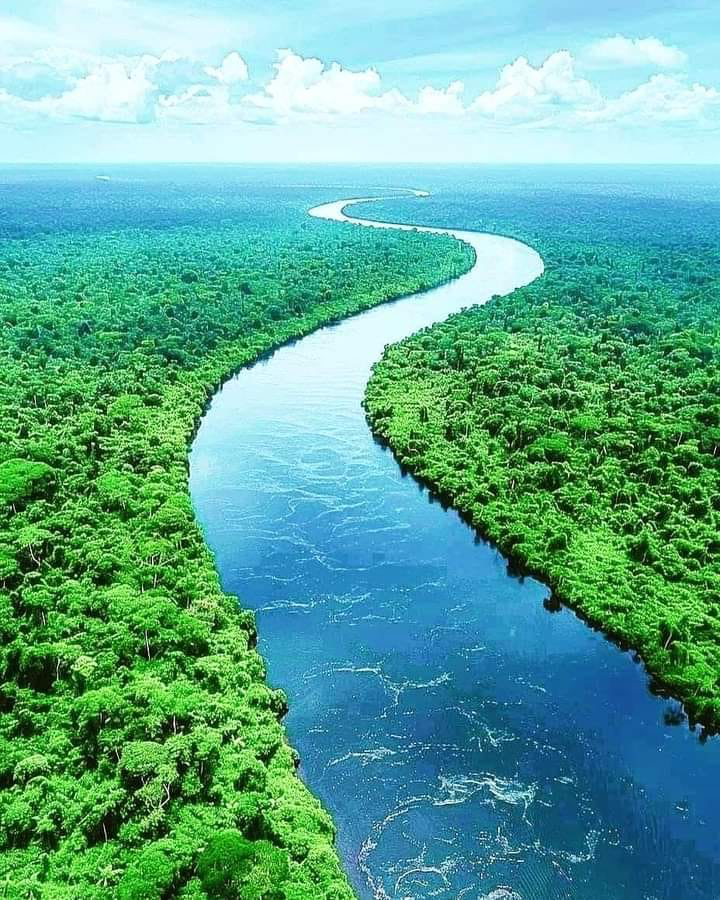
\includegraphics[height=0.4\textheight]{medias/1_/rio_amazonas.png}\hfill
    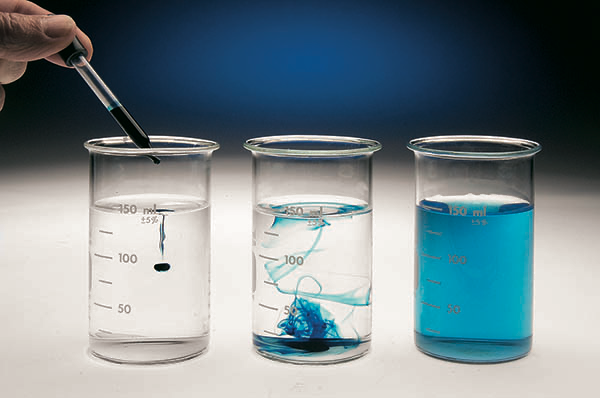
\includegraphics[height=0.4\textheight]{medias/1_/ink_diffusion.png}\hfill
    
\includegraphics[height=0.4\textheight]{medias/1_/chemical_reaction.png}
\end{center}
\pause
    \begin{equation}
        \begin{cases}
            \partial_t u(x,t) = 
                \overbrace{\underbrace{A u}_{c \partial_x u}}^{\text{Advection}}+ 
                \overbrace{\underbrace{D u}_{\partial_x(\eta \partial_x u)}}^{\text{Diffusion}}+ 
                \overbrace{\underbrace{R(u)}_{\text{Non-lin.}}}^{\text{Réaction}},\\[4pt]
            u(x,0)=u_0.
        \end{cases}
    \end{equation}

\end{frame}
  \begin{frame}{Difficultés intrinsèques}{Équations d'ADR}
% \begin{columns}[c,onlytextwidth]

    % ---- Colonne 1 : Opérateurs ----
    % \column{0.67\textwidth}
    \noindent\color{Primary}\rule{\linewidth}{0.6pt}\color{black}\\
    % ---- Colonne 2 : Multi-échelle ----
    % \column{0.30\textwidth}
    \textbf{Des solutions multi-échelles}\\[0.5em]
    \begin{itemize}
        \item plusieurs échelles de temps :\\
        \begin{itemize}
            \item chimie complexe $\tau \sim 50\mathrm{ns}$,\\
            \item advection $\mathrm{Mach }2$ sur $50\mathrm{cm}$ : $\tau \sim 10\mathrm{ms}$.
        \end{itemize}
        \item plusieurs échelles d'espace
    \end{itemize}\pause
    \noindent\color{Primary}\rule{\linewidth}{0.6pt}\color{black}\\
    \textbf{L'intégration conjointe des opérateurs}\\[0.5em]
    Les trois opérateurs ont des propriétés très différentes :
    \begin{itemize}
        \item Advection : Peu raide, raisonnant (spectre autour de $i\mathbb R$).
        \item Diffusion : Moyennement raide, spectre autour de $\mathbb R^-$.
        \item Réaction :  Très raide, hautement non-linéaire, local.
    \end{itemize}
    $\implies$ les approches monolithiques peinent.
\end{frame}

  \begin{frame}{Équations d'ADR}{Stratégies de simulation}
    \textbf{Stratégie $n^o1$ : Différencier le traitement sur chaque opérateurs}\\
        Ne pas faire un schéma monolithique.
        \begin{itemize}
            \item Séparation d'opérateurs (\emph{splitting})
            \item Méthodes ImEx (Additive Runge et Kutta)
        \end{itemize}
        \pause
\noindent\color{Primary}\rule{\linewidth}{0.6pt}\color{black}

    \textbf{Stratégie $n^o2$ : Adaptation en espace}\\
        La multirésolution adaptative : 
        \begin{itemize}
            \item Des grilles de \emph{résolution multiples},
            \item Deux opérateurs de \emph{projection/reconstruction},
            \item Représentation de la solution comme une suite de \emph{détails},
            \item Une stratégie d'\emph{adaptation}.
        \end{itemize}
    \color{red}\begin{figure}[htbp]
    \centering
\begin{tikzpicture}


\node[anchor=west] at (-6.5, -.25) {Niveau $j+1$};
\node[anchor=west] at (-6.5, .25) {Niveau $j$};
\node[anchor=west] at (-6.5, .75) {Niveau $j-1$};
% Niveau j-1

\draw (-4,.5) rectangle (0,1);
\draw (0,.5) rectangle (4,1);

    % Niveau j
\draw (-4,0) rectangle (-2,.5);
\draw (-2,0) rectangle (0,.5);
\draw (0,0) rectangle (2,.5);
\draw (2,0) rectangle (4,.5);
%\node at (1,1.75) {$k=2$};

% Niveau j+1

\draw (-4,-.5) rectangle (-3,0);
\draw (-3,-.5) rectangle (-2,0);
\draw (-2,-.5) rectangle (-1,0);
\draw (-1,-.5) rectangle (0,0);
\draw (0,-.5) rectangle (1,0);
\draw (1,-.5) rectangle (2,0);
\draw (2,-.5) rectangle (3,0);
\draw (3,-.5) rectangle (4,0);

% Relations
\node at (-2, .75) {$k=0$};
\node at (+2, .75) {$k=1$};

\node at (-3, .25) {$k=0$};
\node at (-1, .25) {$k=1$};
\node at (+1, .25) {$k=2$};
\node at (+3, .25) {$k=3$};

\node at (-3.5, -.25) {$k=0$};
\node at (-2.5, -.25) {$k=1$};
\node at (-1.5, -.25) {$k=2$};
\node at (-0.5, -.25) {$k=3$};

\node at (+0.5, -.25) {$k=4$};
\node at (+1.5, -.25) {$k=5$};
\node at (+2.5, -.25) {$k=6$};
\node at (+3.5, -.25) {$k=7$};


\end{tikzpicture}
\caption{Exemple de grille dyadique}
\label{fig:schema_sdyadique}
\end{figure}
\end{frame}
\section{Objectifs}
\begin{frame}{Présentation des contribution}
\end{frame}
\section{$1^{\text{ère}}$ contribution}
  Ce préambule mathématique présente divers concepts innervant dans les travaux du stage (chapitre \ref{par:contrib}). Le lecteur habitué peut ignorer ce chapitre et 
le consulter ponctuellement au besoin. Les sujets suivants y sont introduits:
\begin{enumerate}
    \item
    \item
    \item
    \item
    \item
\end{enumerate}
  \begin{frame}{Comparaison ImEx - Splitting | Nagumo}
\end{frame}
  \begin{frame}{Présentation des méthodes}{Contribution 1 | Comparaison ImEx - Splitting}

\noindent\color{Primary}\rule{\linewidth}{0.6pt}\color{black}\\
\textbf{Méthode ImEx232:\\}
Schéma à trois étages explicites et deux étages implicites, avec $\gamma = \tfrac{2-\sqrt{2}}{2}$ et $\delta = -\tfrac{2\sqrt{2}}{3}$ :
\[
\text{Explicite:}\;\begin{array}{c|ccc}
                        0 & 0 & 0 & 0\\
                        \gamma & \gamma & 0 & 0\\
                        1 & \delta & 1-\delta & 0\\ \hline
                        & 0 & 1-\gamma & \gamma
                    \end{array} \quad
\text{Implicite:}\;
                    \begin{array}{c|cc}
                        \gamma & \gamma & 0\\
                        1 & 1-\gamma & \gamma\\ \hline
                        & 1-\gamma & \gamma
                    \end{array}
\]
\pause
\noindent\color{Primary}\rule{\linewidth}{0.6pt}\color{black}\\
\textbf{Méthode ImEx222:\\}
Schéma à deux étages explicites et deux étages implicites, avec $\gamma = \tfrac{2-\sqrt{2}}{2}$ et $\delta = 1 - \tfrac{1}{2\gamma}$ :
\[
\text{Explicite:}\;
\begin{array}{c|ccc}
0 & 0 & 0 & 0\\
\gamma & \gamma & 0 & 0\\
1 & 1-\delta & \delta & 0\\ \hline
 & 1-\delta & \delta & 0
\end{array}
\quad
\text{Implicite:}\;
\begin{array}{c|cc}
\gamma & \gamma & 0\\
1 & 1-\gamma & \gamma\\ \hline
 & 1-\gamma & \gamma
\end{array}
\]
\pause
\noindent\color{Primary}\rule{\linewidth}{0.6pt}\color{black}\\
\textbf{Méthode Splitting:\\}
Splitting de Strang | Réaction : ERK2 (Heun) | Diffusion : SDIRK2 (celle des méthode ImEx).
\end{frame}

  \begin{frame}{Comparaison ImEx - Splitting | Analyse de stabilité}
\end{frame}
  \begin{frame}{Contribution 1 | Comparaison ImEx - Splitting}{Convergence ($\emptyset$ MRA)}
    \begin{textblock*}{40pt}(0.7\paperwidth,0.2\paperheight)
        
\includegraphics[scale=.03]{medias/2_/1_/light_logo.png}
    \end{textblock*}

    \noindent\color{Primary}\rule{\linewidth}{0.6pt}\color{black}\\
    \textbf{Contexte:\\}
    \begin{itemize}
        \item $k=10$, $D=0.1$,
        \item $\Delta x = 2.4 \, 10^{-3}$,
        \item conditions de Neumann au bord (quasi infini).
    \end{itemize}
    \noindent\color{Primary}\rule{\linewidth}{0.6pt}\color{black}\\
    \centering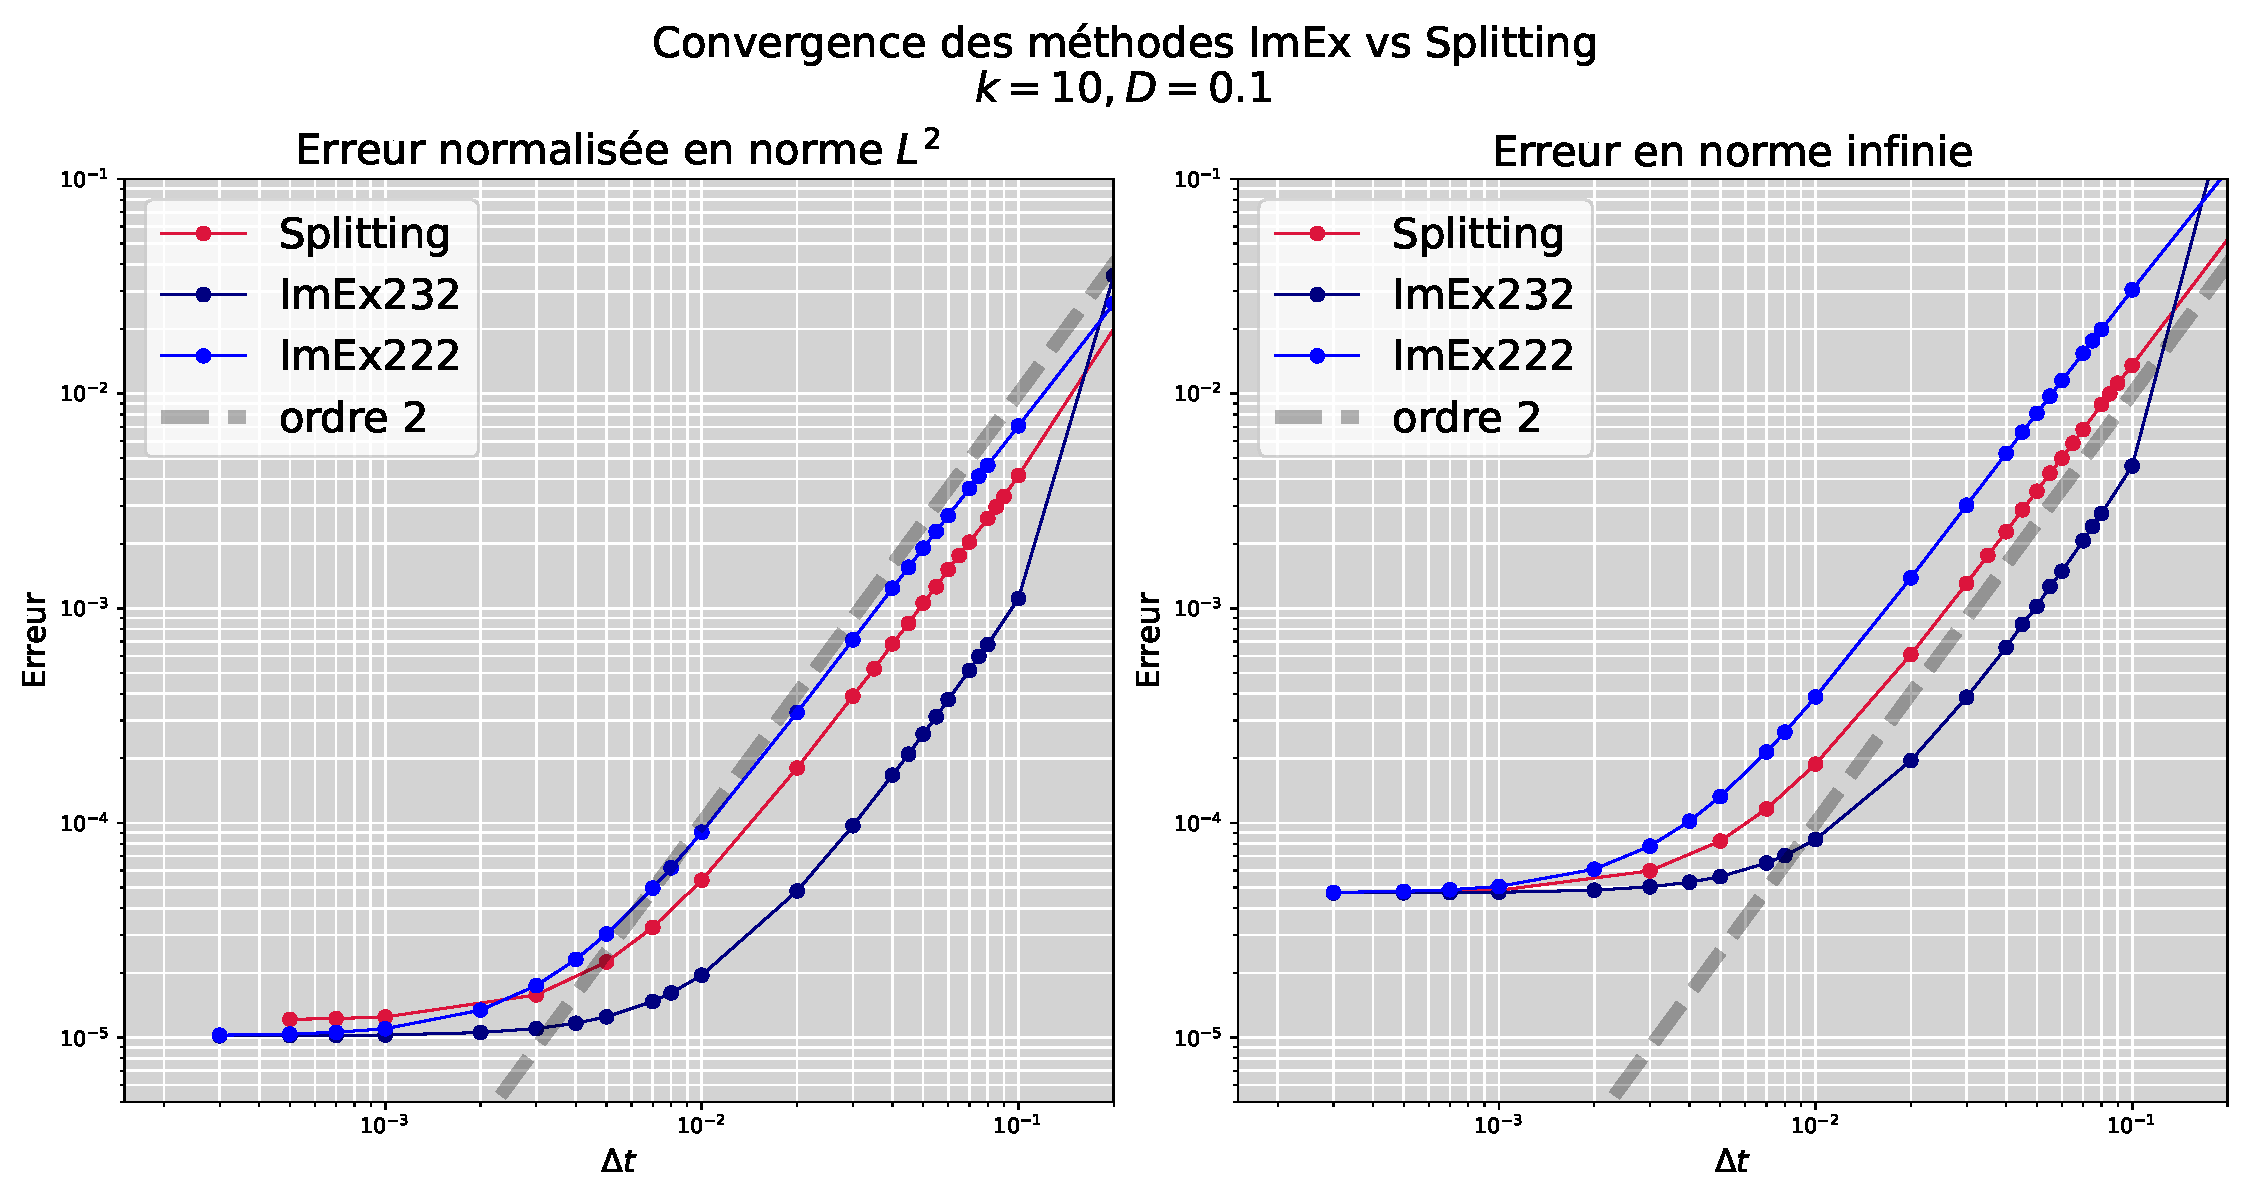
\includegraphics[width =.65 \textwidth]{ medias/2_/1_/ImEx_vs_splitting_k10_D0.1.pdf}
\end{frame}

  \begin{frame}{Contribution 1 | Comparaison ImEx - Splitting}{Convergence (avec MRA)}
    \begin{textblock*}{40pt}(0.7\paperwidth,0.2\paperheight)
        
\includegraphics[scale=.03]{medias/2_/1_/light_logo.png}
    \end{textblock*}
    \noindent\color{Primary}\rule{\linewidth}{0.6pt}\color{black}\\
    \textbf{Contexte:\\}
    \begin{itemize}
        \item $k=10$, $D=0.1$,
        \item Solution représentée du 12 $(\Delta x = 9\, 10^{-3})$ à 6,
        \item conditions de Neumann au bord (quasi infini).
    \end{itemize}   
    \noindent\color{Primary}\rule{\linewidth}{0.6pt}\color{black}\\

    \centering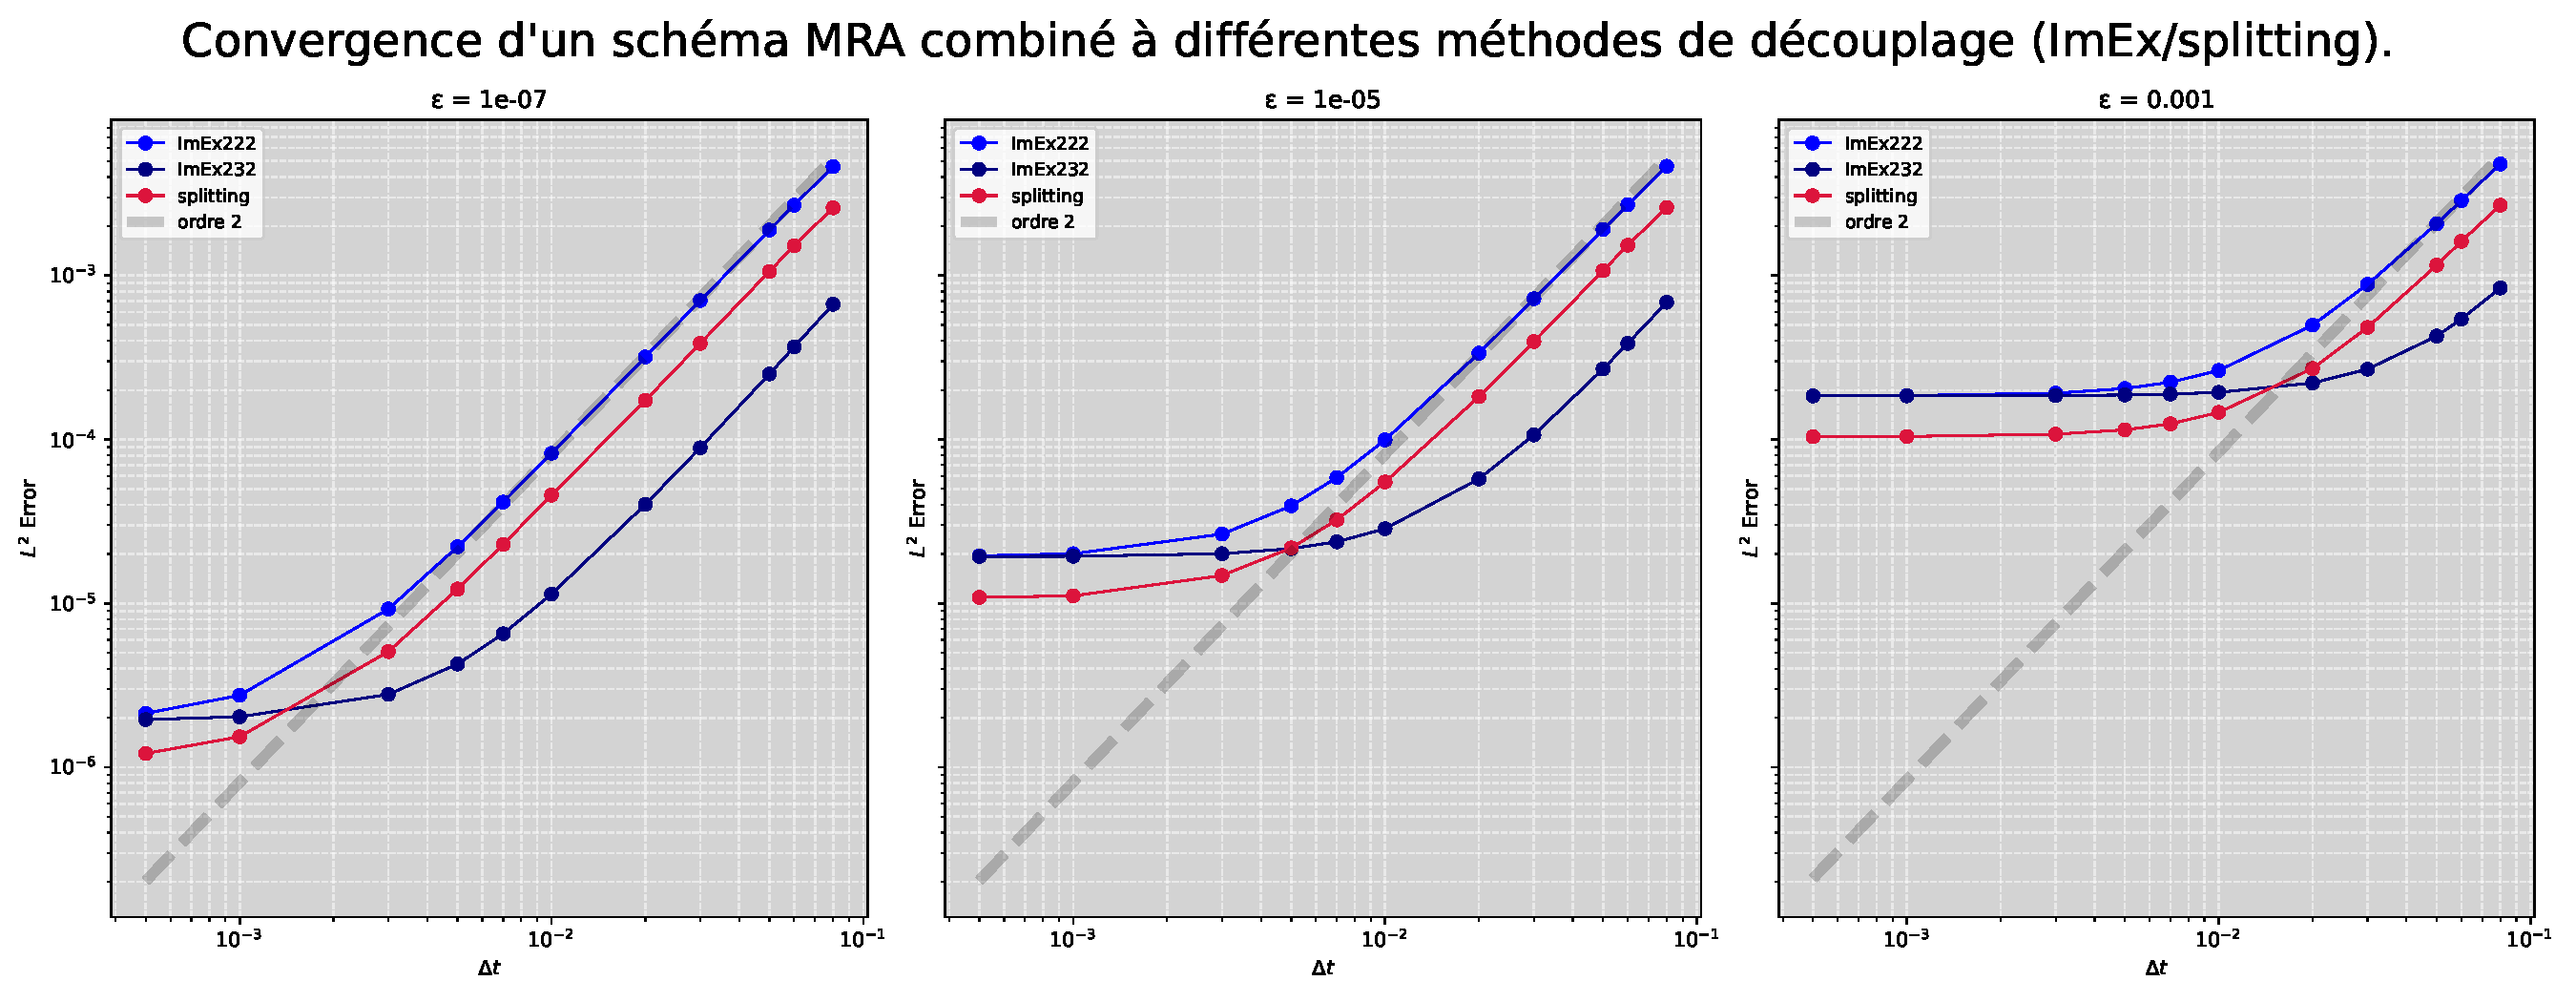
\includegraphics[width = .8\textwidth]{ medias/2_/1_/couplage_MRA_temps_k10_D01.pdf }
\end{frame}
  \input{slides/2_contributions/1_contrib/6_Conclusion}
\section{$2^{\text{nde}}$ contribution}

\end{document}
